Модель Transformer является архитектурой
глубокого обучения, предназначенной для
обработки последовательных данных,
таких как тексты или временные ряды.
Она была предложена в статье \cite{vaswani2017attention} 
и стала одной из самых инновационных архитектур
в области обработки естественного языка.


\begin{figure}[h]
    \centering
    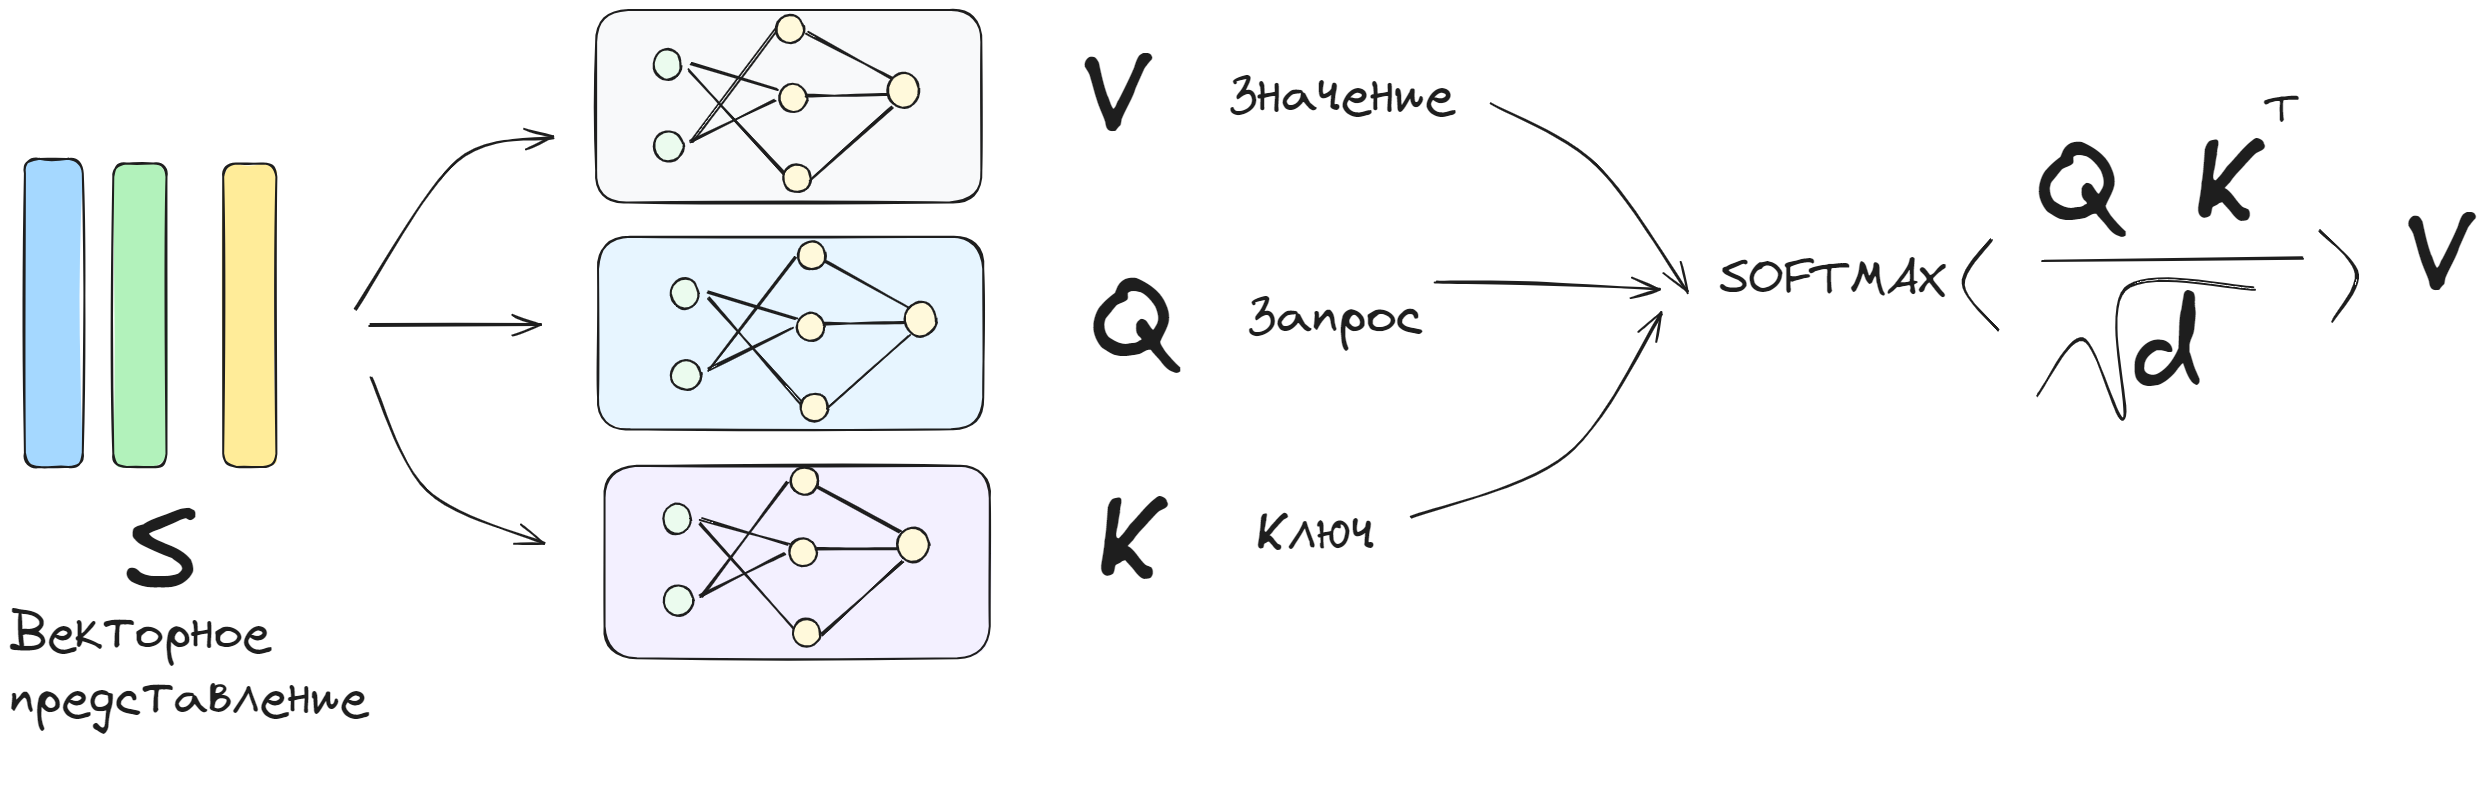
\includegraphics[width=0.5\textwidth]{assets/pedagogic/ml/nn/attention.excalidraw.png}
    \caption{Механизм собственного внимания (Self Attention) \cite{vaswani2017attention} }
    \label{self_attention}
\end{figure}

Механизм внимания (attention) в генеративном моделировании естественного языка является ключевым компонентом в нейронных сетях, 
позволяющим модели фокусироваться на определенных частях входных данных при выполнении задач обработки текста. 
Этот механизм позволяет модели адаптироваться к различным контекстам и динамически выделять важные элементы во входных последовательностях.

Формально, предположим, что у нас есть входные данные \( X = (x_1, x_2, ..., x_T) \) и контекст \( C \), а также текущее состояние скрытого слоя модели \( h_t \). Механизм внимания вычисляет вектор внимания \( \alpha \), который определяет важность каждого элемента входной последовательности на текущем временном шаге:

\[ \alpha_t = \text{softmax}(f(h_t, X)) \]

где \( f \) - функция, которая вычисляет важность каждого элемента входной последовательности, а \( \text{softmax} \) применяется для получения нормированных весов внимания.


\begin{figure}[h]
    \centering
    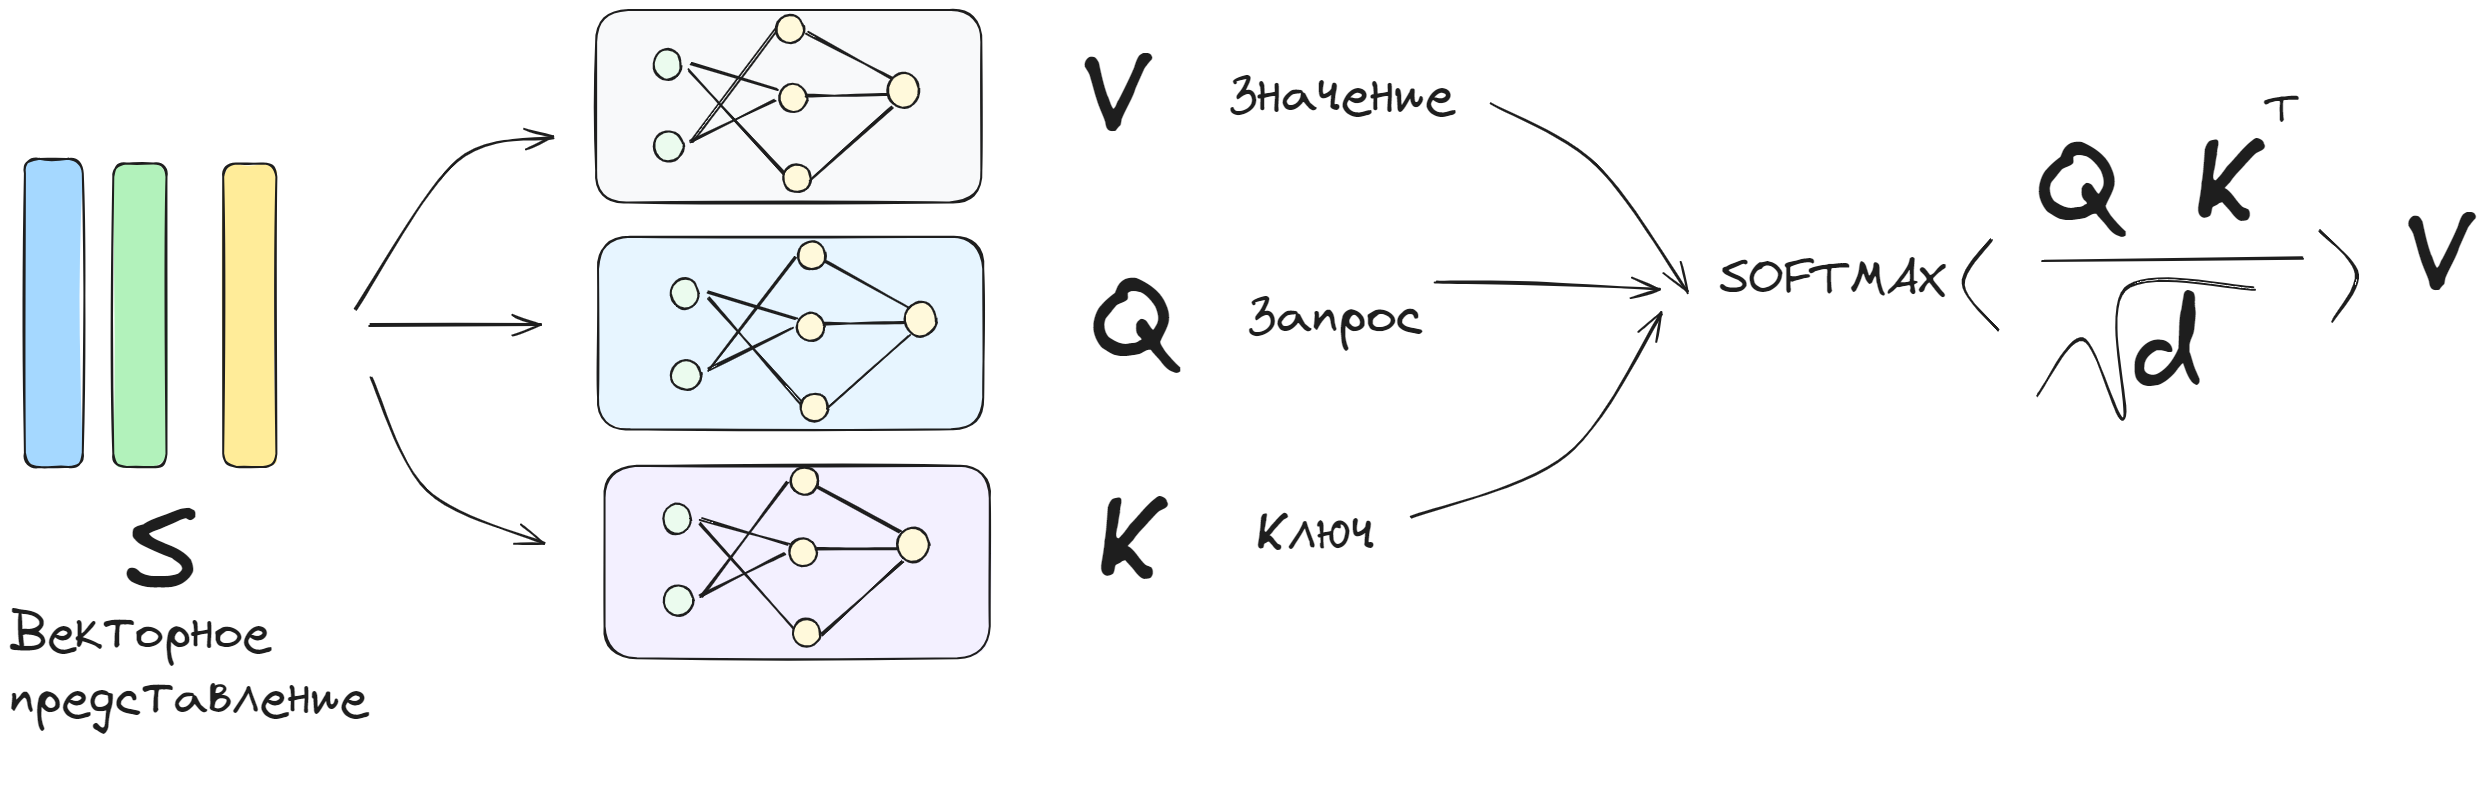
\includegraphics[width=0.5\textwidth]{assets/pedagogic/ml/nn/attention.excalidraw.png}
    \caption{Механизм перекрестного внимания (Cross Attention) \cite{vaswani2017attention} }
    \label{cross_attention}
\end{figure}


Полученный контекст используется в дальнейших вычислениях модели для выполнения задач, таких как генерация текста или классификация.

Механизм внимания позволяет модели сосредоточиться на наиболее значимых частях входных данных в каждый момент времени, что делает его особенно полезным для задач, требующих адаптивности и контекстного понимания, таких как машинный перевод, генерация текста и вопросно-ответные системы. Этот механизм стал ключевым инструментом в области генеративного моделирования естественного языка, позволяя моделям эффективно работать с различными типами данных и контекстами.






Уточним 

 масштабном использовании

Основной компонент модели Transformer 
это механизм внимания (Attention Mechanism).


и

Работа не

Он позволяет модели сосредоточиться 
на наиболее важных частях входных данных при выполнении задач, таких как машинный перевод или обработка текста.

Подробнее опишем механизм внимания.

Каждый 

Нормировка на $\sqrt{d}$.


Механизм внимания в Transformer состоит из трех основных частей:

1. Query, Key, Value (QKV): Это три набора весов, которые модель изучает во время обучения. Они используются для вычисления весов входных данных и определения их важности для каждого элемента. Формально, для каждого элемента \(x_i\) во входных данных, вычисляются query \(q_i\), key \(k_i\) и value \(v_i\) векторы:
$$

 q_i = x_iW_q, \]
\[ k_i = x_iW_k, \]
\[ v_i = x_iW_v, \]
$$
где \(W_q\), \(W_k\), \(W_v\) - матрицы весов, которые модель обучает.

2. Attention Scores: После вычисления query и key векторов, для каждого элемента \(x_i\) вычисляются attention scores \(e_{ij}\) по формуле:

\[ e_{ij} = \frac{q_i \cdot k_j}{\sqrt{d_k}}, \]

где \(d_k\) - размерность ключевого (или запросового) пространства. Этот шаг позволяет модели оценить важность каждого элемента входных данных для каждого другого элемента.

3. Веса внимания (Attention Weights): Attention scores преобразуются в веса внимания \( \alpha_{ij} \) с помощью функции softmax:

\[ \alpha_{ij} = \frac{\exp(e_{ij})}{\sum_{j'} \exp(e_{ij'})}. \]

Эти веса показывают, какую важность модель придает каждому элементу данных при решении конкретной задачи. 

После вычисления весов внимания, они умножаются на соответствующие значения (value) и суммируются, чтобы получить итоговый взвешенный вектор, который представляет собой выход механизма внимания.

Механизм внимания в Transformer может быть использован в нескольких вариантах: внутри блоков кодировщика и декодировщика для обработки последовательных данных в машинном переводе, внутри блоков самовнимания (self-attention) для обработки последовательных данных в других задачах, таких как генерация текста или анализ сентимента.

Таким образом, механизм внимания в модели Transformer позволяет ей эффективно обрабатывать и анализировать последовательные данные, учитывая их важность и контекст.
